\begin{figure*}[b]
    \centering
    \begin{subfigure}{.5\textwidth}
        \centering
        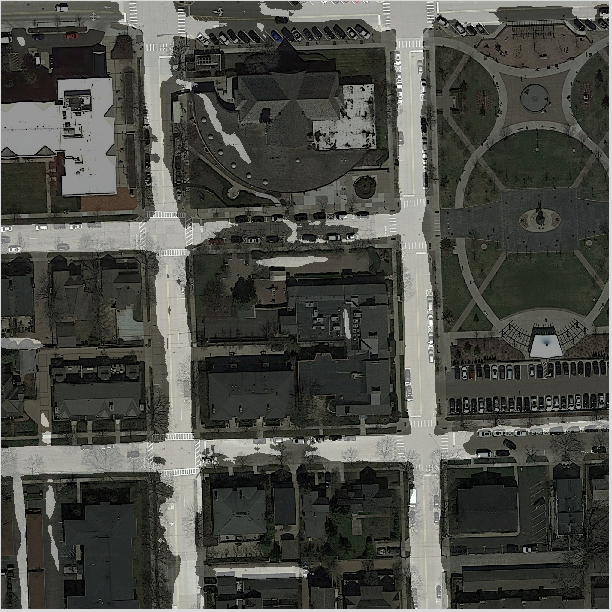
\includegraphics[width=.65\linewidth]{images/baseline_test_136.png}
        \caption{Baseline}%
        \label{fig:res_before}
    \end{subfigure}%
    \begin{subfigure}{.5\textwidth}
        \centering
        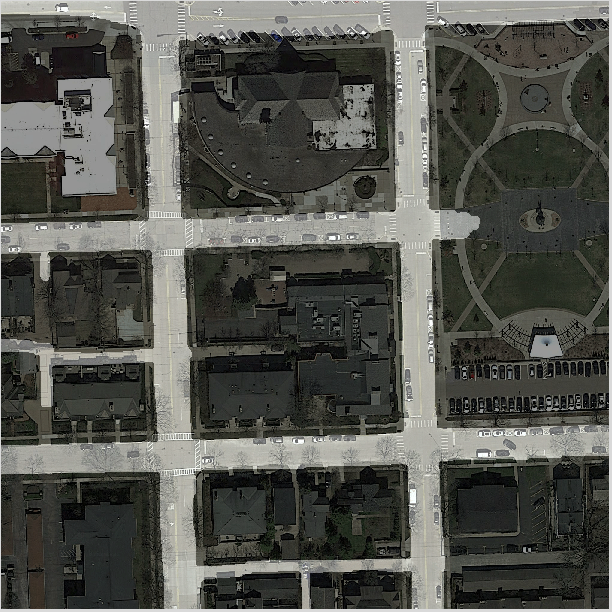
\includegraphics[width=.65\linewidth]{images/final_test_136.png}
        \caption{Final}%
        \label{fig:res_after}
    \end{subfigure}
    \caption{%
        Comparison of the baseline model with our final one.
        The output is binarized and overlaid on top of the input.
    }
\end{figure*}

Table \ref{results:metrics} highlights the results using the different novelties. The rows are arranged in the order of application --- we start with the baseline, and then apply our augmentations, contrastive learning, and so on.
Note that the test accuracy is calculated from the public Kaggle leaderboard, which uses the downsampled outputs.

\begin{table}[ht]
    \centering
    \caption{
        Comparison of results of all novelties.
        Each novelty is applied with all previous novelties.
    }%
    \label{results:metrics}
    \begin{tabular}{l r r r} 
        \toprule
        Method & Train Acc & Val Acc & Test Acc \\
        \midrule
        Baseline & 0.99132 & 0.96531 & 0.89714 \\ 
        + Aug & 0.97889 & 0.96470 & 0.91352 \\
        + CL & 0.97806 & 0.96230 & 0.91638 \\
        + Cleaned data & 0.97932 & 0.96394 & 0.92022 \\
        + Graph Cut & 0.97923 & 0.96327 & 0.91832 \\
        + SPP & 0.97936 & 0.96388 & \textbf{0.92144} \\
        \bottomrule
    \end{tabular}
\end{table}

Applying Graph Cut directly reduces the test accuracy, and decreases final accuracy as opposed to only applying SPP.
Still, we decide to submit this version, since the difference is minimal and the outputs show more sensible street classifications.
It is important to note, that these two post-processing algorithms are training data agnostic, and therefore they do not improve that metric.

Figure~\ref{fig:res_before} displays a sample output from the baseline model.
The corresponding image by our final model is shown in Figure~\ref{fig:res_after}.
It is visible how much our novelties improve over the baseline model, especially in the connectivity of streets.